\documentclass[slide,papersize,fleqn,22pt]{jsarticle}
\usepackage[dvipdfmx]{graphicx,color}
\pagecolor[rgb]{0.8,0.8,1}
\usepackage[T1]{fontenc}
\usepackage{textcomp}
\renewcommand{\rmdefault}{ptm}
\usepackage[scaled]{helvet}
\renewcommand{\ttdefault}{pcr}
\usepackage{tikz}
\usetikzlibrary{arrows,decorations.pathmorphing,backgrounds,positioning,fit,shapes}
\usepackage{tcolorbox}
\usepackage{amsmath,amssymb}
\usepackage{exscale}
\usepackage{multicol}
\usepackage{url}
\begin{document}
\西暦
\title{構文解析系を書いてみよう}
\author{R\&D center\\別所 博之}
\maketitle
\section{構文解析系?}
言語処理系 (コンパイラ、インタプリタ) の中で、ソースコードを文法に従っ
て解析する部分
\section{言語処理系の内部構成}
コンパイラの内部構成の例
\newcommand{\figureA}{%
\begin{tikzpicture}[
    node distance=0.5cm,auto,
    object/.style={font=\tiny},
    anchor/.style={font=\tiny},
    subcompo/.style={rectangle,draw=black!50,fill=black!20,thick,font=\tiny,align=center}
  ]
  \node[object,font=\tiny,align=center] (sourcecode) {ソースコード\\(文字列)};
  \node[object] (P1) [right=of sourcecode] {};
  \node[object] (tokens) [right=of P1] {トークン列};
  \node[object] (P2) [right=of tokens] {};
  \node[object] (tree) [right=of P2] {構文木};
  \node[object] (P3) [right=of tree] {};
  \node[object] (objectcode) [right=of P3] {機械語};
  \node[subcompo] (lexer) [above=of P1] {字句解析\\lexical analyzer};
  \node[subcompo] (parser) [above=of P2] {構文解析\\parser};
  \node[subcompo] (generator) [above=of P3] {コード生成\\code generator};
  \node[subcompo] (optimizer) [below=of generator] {Optimizer};

  \path (sourcecode) edge[->] (lexer);
  \path (lexer) edge[->] (tokens);
  \path (tokens) edge[->] (parser);
  \path (parser) edge[->] (tree);
  \path (tree) edge[->] (generator);
  \path (generator) edge[->] (objectcode);
  \path (generator) edge (optimizer);

  \node[draw=red,fit=(tokens) (lexer) (parser),ellipse] {};
\end{tikzpicture}}
\figureA
\section{何のために?}
\small
構文解析系を学ぶべき理由
\begin{itemize}
\item プログラミングの学習題材として
  \begin{itemize}
  \item 構文解析は、'50〜'70年代くらいに盛んに研究されて、現在では枯れた分野
  \item 情報学科のカリキュラムや、参考書などに取り上げられることが多い
  \end{itemize}
\item 使っている道具(コンパイラとか)を理解する 
\item 言語の文法の形式定義を理解できる \\
  => 新しい言語の習得が速くなる
\item アプリケーションに拡張機能を持たせる
  \begin{itemize}
  \item マクロ動作、プラグインなど \\
    \begin{itemize}
      \item AutoLisp (AutoCAD)
      \item VBA (Excel)
      \item Tera Term マクロ
    \end{itemize}
  \item 設定ファイルの記述力を強化する
  \end{itemize}
  {\tiny (この目的には、俺言語より埋め込み用言語 (Lua, Javascript, Tclなど) の
  方が向いている)}
\end{itemize}
とか、色々あるけど…
\section{何のために?}
\begin{tcolorbox}
  \Large
  プログラマたるもの一生に一度くらい、俺言語を作ってみたいよね! (Y/y)?
\end{tcolorbox}
\begin{flushright}
実際に作るかはともかく、心意気として…
\end{flushright}
\section{IT業界の強者は作ってきた}
\begin{tabular}{ll}
  Sun Microsystems & Java \\
  Netscape & Javascript \\
  Apple & Swift \\
  Google & Go \\
  Mozilla & Rust
\end{tabular}
\section{閑話休題}
\figureA
\section{例題}
有理数の四則演算を実行する計算機を作れ
\tiny
\begin{tcolorbox}[box align=center,width=0.5\hsize,nobeforeafter]
  \texttt{1/6 + 1/6}
\end{tcolorbox}
{$\Rightarrow$}
\begin{tcolorbox}[box align=center,width=0.4\hsize,nobeforeafter]
\texttt{1/3}
\end{tcolorbox}
\vfill
変数が使えること。
\vfill
\begin{tcolorbox}[box align=center,width=0.5\hsize,nobeforeafter]
\begin{verbatim}
nearly_pie = 355/113
r = 15
nearly_pie * r * r
\end{verbatim}
\end{tcolorbox}
{$\Rightarrow$}
\begin{tcolorbox}[box align=center,width=0.4\hsize,nobeforeafter]
\texttt{ 79875/113}
\end{tcolorbox}
\vfill
. コマンドで浮動小数点の近似値を表示する
\vfill
\begin{tcolorbox}[box align=center,width=0.5\hsize,nobeforeafter]
\texttt{. nearly\_pie * r * r}
\end{tcolorbox}
{$\Rightarrow$}
\begin{tcolorbox}[box align=center,width=0.4\hsize,nobeforeafter]
\texttt{706.85840707965}
\end{tcolorbox}
\normalsize
\section{おさらい有理数}
有理数 (Rational number)

$\mathbb{Q} = \left\{{a \over b} \mid a, b \in \mathbb{Z}, b\ne
0\right\}$
($\mathbb{Z}$ は整数の集合)
\vspace{1em}

二つの整数 $a, b$ (ただし $b \ne 0$) を用いて、$a/b$ の形で表せる数

\section{C言語で定義するなら}
\tiny
\begin{verbatim}
typedef struct rational {
  long numerator;
  long denominator;
} Rational;

Rational rational_new(long, long);
Rational rational_add(Rational, Rational);  
Rational rational_sub(Rational, Rational);  
Rational rational_mul(Rational, Rational);  
Rational rational_div(Rational, Rational);
...
\end{verbatim}
\normalsize

Ruby、Python には Rationalクラスがある。

C++ は、boost に rational クラスがある。

\section{文法を定義する}
\small
プログラミング言語の文法を定義するには、\textbf{BNF}
(\textsl{Backus-Naur form\/}) を使う。
\begin{itemize}
\item 文脈自由文法を定義するためのメタ言語。
\item John Buckus と Peter Naur が、ALGOL60 の文法を定義するために考案。
\end{itemize}
\begin{description}
\item[定義] $A \rightarrow B$  (A は Bである)
\item[連接] $A \rightarrow B\,C$ (A は B に C が続いたものである)
\item[選択] $A \rightarrow B\,|\,C$ (A は B または C である)
\end{description}

\section{BNFによる識別子の定義}
\begin{tcolorbox}[nobeforeafter]
  \tiny
英字、数字、`\_' が1文字以上連続したもの。ただし、先頭は数字でない。
\end{tcolorbox}
\newcommand{\OR}{\quad|\quad}%
\newcommand{\q}{\quad}%
\footnotesize
\begin{gather*}
\textit{identifier} \rightarrow \textit{idchar1}\quad
\textit{identifier2} \\
\textit{identifier2} \rightarrow \texttt{""}\OR\textit{idchar2}\quad
\textit{identifier2} \\
\textit{idchar1}\rightarrow\textit{alphabet}\OR\texttt{"\_"} \\
\textit{idcahr2}\rightarrow\textit{idchar1}\OR\textit{digit} \\
\textit{digit}\rightarrow\texttt{"0"}|\texttt{"1"}|\texttt{"2"}|\texttt{"3"}|\texttt{"4"}|\texttt{"5"}|\texttt{"6"}|\texttt{"7"}|\texttt{"8"}|\texttt{"9"}
\end{gather*}
\tiny\vfill
\textit{identifier2}の再帰定義によって繰り返しを表現している。
\normalsize
\section{EBNF}
Extended BNF
\begin{description}
\item[0回以上の繰り返し] $A*$
\item[1回以上の繰り返し] $A+$
\item[省略可能] $A?$
\item[グループ化] $(A)$
\item[0回以上の繰り返し] $\{A\}$
\item[省略可能] $[A]$
\item[省略可能] $A_{opt}$
\end{description}

\section{EBNFによる識別子の定義}
\[
\footnotesize
\textit{identifier} \rightarrow (\textit{alphabet}\,|\texttt{"\_"})\quad(\textit{alphabet}\,|\texttt{"\_"}|\textit{digit})*
\]

\tiny
( $^oд^o$) ただの正規表現ですね
\normalsize
\section{EBNFの使用例}
\begin{itemize}
\item C
  \begin{itemize}
  \item K\&R の巻末
  \item ISO/JIS 規格票
  \end{itemize}
\item Python {\tiny(\url{https://docs.python.org/3/reference/grammar.html})}
\item W3C {\tiny(\url{https://www.w3.org/})}
\end{itemize}



\section{ABNF}
Augmented BNF
\begin{itemize}
\item RFC 5234
\item 各種RFCで、定義を記述するためのBNF
\item 使用例
  \begin{description}
  \item[RFC3986] URIの定義
    \item[RFC2822] Internet Message Format
  \end{description}
\end{itemize}

\section{BNFに関連する用語}
\begin{description}
\item[文脈自由文法] (context-free grammer) \\
  BNFで表現できるのは、「文脈自由文法」クラスに属する文法である。
\item[導出]
  $\rightarrow$ の左辺のアイテムから右辺のアイテムに変換する作業を「導
  出」と呼ぶ。
\item[終端記号] BNFの$\rightarrow$ の右辺にしか表れないアイテムを「終
  端記号」と呼ぶ。左辺にも表れるアイテムは「非終端記号」である。
\end{description}

\section{Railroad Diagram}
\tiny
\begin{gather*}
  \textit{floating point number} \rightarrow \\
  \textit{unsigned integer}\q
(\texttt{"."}\q\textit{digit}+)? \q (\texttt{"E"}\q(\texttt{"+"}|\texttt{"-"})?
\textit{unsigned integer})?
\end{gather*}
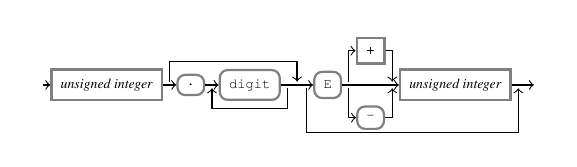
\begin{tikzpicture}[
    point/.style={circle,inner sep=0pt,minimum size=2pt},
    nonterminal/.style={draw=black!50,thick,rectangle,font=\itshape\tiny},
    terminal/.style={draw=black!50,thick,rectangle,rounded
      corners=1mm,font=\ttfamily\tiny},
    skiploop/.style={to path={-- ++(0,#1) -| (\tikztotarget)}},
    hvpath/.style={to path={-| (\tikztotarget)}},
    vhpath/.style={to path={|- (\tikztotarget)}}
  ]
  \matrix[row sep=0.5mm,column sep=0.5mm] {
    & & & & & & & & & & & & \node (plus) [nonterminal] {+}; & \\
    \node (p1) [point] {}; & & \node (ui1) [nonterminal] {unsigned integer}; &
    \node (p2) [point] {}; & \node (dot) [terminal] {.}; &
    \node (p3) [point] {}; & \node (digit) [terminal]{digit}; &
    \node (p4) [point] {}; & \node (p5) [point] {}; &
    \node (p6) [point] {}; & \node (e) [terminal] {E}; &
    \node (p7) [point] {}; & &
    \node (p8) [point] {}; & \node (ui2) [nonterminal] {unsigned integer}; &
    \node (p9) [point] {}; & \node [point] (p10) {}; &
    \node [point] (p11) {};\\
    & & & & & & & & & & & & \node (minus) [terminal] {-}; & \\
  };

  \path (p1) edge [->] (ui1);
  \path (ui1) edge [->] (dot);
  \path (dot) edge [->] (digit);
  \path (digit) edge [->] (e);
  \path (e) edge [->] (ui2);
  \path (ui2) edge [->] (p11);
  \path (p7) edge [->,vhpath] (plus) (plus) edge [->,hvpath] (p8);
  \path (p7) edge [->,vhpath] (minus) (minus) edge [->,hvpath] (p8);
  \path (p4) edge [->,skiploop=-3mm] (p3)
  (p2) edge [->,skiploop=3mm] (p5)
  (p6) edge [->,skiploop=-6mm] (p9)
  ;
\end{tikzpicture}

\begin{itemize}
\item Railroad Diagram Generator: \url{http://www.bottlecaps.de/rr/ui}
\end{itemize}

\section{BNFの意義}
\footnotesize
BNFの登場により、
\begin{enumerate}
\item 言語の文法を形式的に定義できるようになり、曖昧さがなくなった。
  \begin{itemize}
  \item ALGOL60以前は、自然言語によってプログラミング言語の文法を定義
    していた。
  \item 言語 (人工言語と自然言語を含む)の性質が研究され、機械にも人間
    にも解釈しやすいプログラミング言語の文法が定義されるようになった。
  \end{itemize}
\item 構文解析系を自動生成する道が開けた。
  \begin{itemize}
  \item compiler-compiler (BNFを入力として、パーザを生成する)
  \end{itemize}
\end{enumerate}

\section{有理数計算機の文法定義}
\newcommand{\T}[1]{\texttt{"#1"}}%
\setlength{\abovedisplayskip}{1pt}%
\setlength{\belowdisplayskip}{1pt}%
\tiny
\multicolsep=0pt
\begin{multicols}{2}
\begin{align*}
文 \rightarrow & 式\q 行末 \OR \\
& \textrm{/* 代入文 */} \\
& 識別子\q\T=\q 式\q 行末 \OR\\
& \texttt{"."}\q 式\q 行末
\end{align*}
\begin{gather*}
行末\rightarrow \textit{LF}\q \textrm{/* ASCII 0x0a*/} \OR
\textit{EOF} \\
識別子\rightarrow (英字|\T\_)\q (英字|\T\_|数字)* \\
数\rightarrow 数字\texttt{+}\q \textrm{/*正整数*/}
\end{gather*}
\begin{align*}
  式\rightarrow & 識別子 \OR 数 \OR\\
  & \texttt{"("}\q 式\q\texttt{")"} \OR \\
  & 単項演算子 \q 式 \OR \\
  & 式\q 二項演算子\q 式
\end{align*}
\begin{align*}
  単項演算子\rightarrow & \T- \\
  二項演算子\rightarrow & \T+\OR\T-\OR\\
  & \T*\OR\T/ \\
  空白文字\rightarrow& \T{ } \textrm{/*ASCII 0x20*/}\OR \\
  & タブ \textrm{/*ASCII 0x09*/} \OR \\
  & \textit{CR} \textrm{/* ASCII 0x0d*/} \\
  空白\rightarrow &空白文字\texttt{+} \\
  \intertext{/*トークンの間の空白は無視する*/} \\
  \intertext{/*数字と英字の定義は省略*/}
\end{align*}
\end{multicols}
\normalsize

\section{字句解析}
\begin{tikzpicture}[
    node distance=0.5cm,auto,
    object/.style={font=\tiny},
    anchor/.style={font=\tiny},
    subcompo/.style={rectangle,draw=black!50,fill=black!20,thick,font=\tiny,align=center}
  ]
  \node[object,font=\tiny,align=center] (sourcecode) {ソースコード\\(文字列)};
  \node[object] (P1) [right=of sourcecode] {};
  \node[object] (tokens) [right=of P1] {トークン列};
  \node[object] (P2) [right=of tokens] {};
  \node[object] (tree) [right=of P2] {構文木};
  \node[object] (P3) [right=of tree] {};
  \node[subcompo] (lexer) [fill=red!20,above=of P1] {字句解析\\lexical analyzer};
  \node[subcompo] (parser) [above=of P2] {構文解析\\parser};

  \path (sourcecode) edge[->] (lexer);
  \path (lexer) edge[->] (tokens);
  \path (tokens) edge[->] (parser);
  \path (parser) edge[->] (tree);
\end{tikzpicture}

\section{字句解析}
\footnotesize
ソースコードをトークンに分割する
\begin{center}
  \texttt{foo = bar[0x10]+++baz;} \\
  $\Downarrow$ \\
  \fbox{foo}~
  \fbox{=}~
  \fbox{bar}~
  \fbox{[}~
  \fbox{0x10}~
  \fbox{]}~
  \fbox{++}~
  \fbox{+}~
  \fbox{baz}~
  \fbox{;}
\end{center}
\begin{itemize}
\item 識別子 (identifier)
  \item 予約語
\item リテラル (literal)
  \begin{itemize}
  \item 数値リテラル
  \item 文字列
  \end{itemize}
\item 演算子 (operator)
\end{itemize}
\section{C言語のプリプロセッサ}
\tiny
\begin{tikzpicture}[
    node distance=0.5cm,auto,
    object/.style={font=\tiny},
    anchor/.style={font=\tiny},
    subcompo/.style={rectangle,draw=black!50,fill=black!20,thick,font=\tiny,align=center}
  ]
  \node[object,font=\tiny,align=center] (sourcecode) {ソースコード\\(文字列)};
  \node[object] (P1) [right=of sourcecode] {};
  \node[object] (tokens) [right=of P1] {トークン列};
  \node[object] (P2) [right=of tokens] {};
  \node[object] (tokens2) [right=of P2] {トークン列};
  \node[object] (P3) [right=of tokens2] {};
  \node[object] (tree) [right=of P3] {構文木};
  \node[subcompo] (lexer) [above=of P1] {字句解析\\lexical analyzer};
  \node[subcompo] (preprocessor) [above=of P2] {マクロ展開\\macro expansion};
  \node[subcompo] (parser) [above=of P3] {構文解析\\parser};

  \path (sourcecode) edge[->] (lexer);
  \path (lexer) edge[->] (tokens);
  \path (tokens) edge[->] (preprocessor);
  \path (preprocessor) edge[->] (tokens2);
  \path (tokens2) edge[->] (parser);
  \path (parser) edge[->] (tree);
\end{tikzpicture}

\textbf{プリプロセッサが別プログラムの場合 }
\begin{tikzpicture}[
    node distance=0.2cm,auto,
    object/.style={font=\tiny,align=center},
    anchor/.style={font=\tiny},
    subcompo/.style={rectangle,draw=black!50,fill=black!20,thick,font=\tiny,align=center}
  ]
  \node[object] (sourcecode) {ソースコード\\(文字列)};
  \node[object] (P1) [right=of sourcecode] {};
  \node[object] (tokens) [right=of P1] {トークン列};
  \node[object] (P2) [right=of tokens] {};
  \node[object] (sourcecode2) [right=of P2] {ソースコード\\(マクロ展開済み)};
  \node[object] (P3) [right=of sourcecode2] {};
  \node[object] (tokens2) [right=of P3] {トークン列};
  \node[object] (P4) [right=of tokens2] {};
  \node[object] (tree) [right=of P4] {構文木};
  \node[subcompo] (lexer1) [above=0.5cm of P1] {字句解析\\lexical analyzer};
  \node[subcompo] (preprocessor) [above=0.5cm of P2] {マクロ展開\\macro expansion};
  \node[subcompo] (lexer2) [above=0.5cm of P3] {字句解析\\lexical analyzer};
  \node[subcompo] (parser) [above=0.5cm of P4] {構文解析\\parser};

  \path (sourcecode) edge[->] (lexer1);
  \path (lexer1) edge[->] (tokens);
  \path (tokens) edge[->] (preprocessor);
  \path (preprocessor) edge[->] (sourcecode2);
  \path (sourcecode2) edge[->] (lexer2);
  \path (lexer2) edge[->] (tokens2);
  \path (tokens2) edge[->] (parser);
  \path (parser) edge[->] (tree);
  \node[draw=red,fit=(lexer1) (preprocessor),rectangle] (cpp) {};
  \node [above=1mm of cpp] {\tiny cpp};
  \node[draw=blue,fit=(lexer2) (parser),rectangle] (cc1) {};
  \node [above=1mm of cc1] {\tiny cc1};
\end{tikzpicture}

\texttt{cc -E} でプリプロセッサの出力を確認できる。

プリプロセッサは C言語の構文について(ほとんど)知らない。

\normalsize
\section{字句解析系の実装}
\url{https://github.com/bsh-git/seminar_parser/}

\texttt{ratcal\_lex.rb}

\section{構文解析}
\begin{tikzpicture}[
    node distance=0.5cm,auto,
    object/.style={font=\tiny},
    anchor/.style={font=\tiny},
    subcompo/.style={rectangle,draw=black!50,fill=black!20,thick,font=\tiny,align=center}
  ]
  \node[object,font=\tiny,align=center] (sourcecode) {ソースコード\\(文字列)};
  \node[object] (P1) [right=of sourcecode] {};
  \node[object] (tokens) [right=of P1] {トークン列};
  \node[object] (P2) [right=of tokens] {};
  \node[object] (tree) [right=of P2] {構文木};
  \node[object] (P3) [right=of tree] {};
  \node[subcompo] (lexer) [above=of P1] {字句解析\\lexical analyzer};
  \node[subcompo] (parser) [fill=red!20,above=of P2] {構文解析\\parser};

  \path (sourcecode) edge[->] (lexer);
  \path (lexer) edge[->] (tokens);
  \path (tokens) edge[->] (parser);
  \path (parser) edge[->] (tree);
\end{tikzpicture}

\footnotesize
よくある実装方法:
\begin{itemize}
\item 上昇型
  \begin{itemize}
  \item 移動還元構文解析 (shift-reduce parser)
  \end{itemize}
\item 下降型
  \begin{itemize}
  \item 再帰降下型構文解析 (recursive descent parser)
  \end{itemize}
\end{itemize}
\normalsize

\section{構文木 (Parse Tree)}
\tiny
作例の計算機程度であれば、構文木を作るのではなくて、構文解析しながら計
算も実行してしまう実装もありだが...

\tcbox[box align=center,nobeforeafter,size=fbox]{%
\texttt{a = 3*b + 42/1984}}
{$\Rightarrow$}
\begin{tcolorbox}[box align=center,width=0.5\hsize,nobeforeafter]
\tikz [sibling distance=6em,level distance=3em,
  level 2/.style={sibling distance=8em},
  level 3/.style={sibling distance=3em}
] \node {代入}
child { node[align=center] {識別子\\a}}
child { node {+}
  child { node {*}
    child { node[align=center] {数\\3}}
    child {node[align=center] {識別子\\b}}}
  child { node {/}
    child { node[align=center] {数\\42}}
    child { node[align=center] {数\\1984}} }
};
\end{tcolorbox}

\section{パーザの実装と実演}
\texttt{ratcal\_parser.rb}\\
\texttt{ratcal\_exec.rb}

\section{演算子の優先度}
\newcommand{\OP}[1]{\,\textit{op}_#1\,}
\[A \OP1 B \OP2 C \OP1 D \]
\tcbox[box align=center,nobeforeafter,size=fbox]{%
$\OP1 > \OP2$}
{$\Rightarrow$}
\tcbox[box align=center,nobeforeafter,size=fbox]{%
$(A \OP1 B) \OP2 (C \OP1 D)$}
{$\Rightarrow$}
\tcbox[box align=center,size=fbox,nobeforeafter]{
\tikz [sibling distance=6em,level distance=3em,
  level 1/.style={sibling distance=5em},
  level 2/.style={sibling distance=2em}
] \node {$op_2$}
child { node {$op_1$}
  child { node {A} }
  child { node {B} }}
child { node {$op_1$}  
  child { node {C} }
  child { node {D} }}; }

\tcbox[box align=center,nobeforeafter,size=fbox]{%
$\OP1 < \OP2$}
{$\Rightarrow$}
\tcbox[box align=center,nobeforeafter,size=fbox]{%
$A \OP1 (B \OP2 C) \OP1$}
{$\Rightarrow$}
\tcbox[box align=center,size=fbox,nobeforeafter]{
\tikz [sibling distance=6em,level distance=3em,
  level 1/.style={sibling distance=5em},
  level 2/.style={sibling distance=2em}
] \node {$op_1$}
child { node {$op_1$}
  child { node {A} }
  child { node {$op_2$}
    child { node {B} }
    child { node {C} }}}
child { node {D} }; }
\section{演算子の結合性}
\renewcommand{\OP}{\,\textit{op}\,}
\setlength{\abovedisplayskip}{-1em}
\[A \OP B \OP C \OP D \]
左結合 $((A \OP B) \OP C) \OP D \Rightarrow$
\tcbox[size=fbox,nobeforeafter]{
  \tikz [sibling distance=3em,level distance=2em
  ] \node {$op$}
  child {node {$op$}
    child { node {$op$}
      child { node {A} }
      child { node {B} }}
    child { node {C} }}
  child {node {D}}; }

右結合 $A \OP (B \OP (C \OP D)) \Rightarrow$
\tcbox[size=fbox,nobeforeafter]{
\tikz [sibling distance=3em,level distance=2em
] \node {$op$}
child { node {A} }
child { node {$op$}
  child { node {B} }
  child { node {$op$}
    child { node {C}}
    child { node {D}} } }; }
\section{優先度と結合性とBNF}
\normalsize
優先度と結合性を定義するには:
\begin{itemize}
\item BNFには書かずに、追加仕様として演算子毎の優先度と結合性を与える
  \begin{itemize}
  \item Shift-reduce パーザや、compiler-compiler 向き
  \end{itemize}
\item BNFで優先度と結合性を表現する
  \begin{itemize}
  \item 再帰降下パーザ向き
  \end{itemize}
\end{itemize}

\section{BNFで優先度を表現する}
「式」を優先度毎に細かく分割する
\tiny
\begin{align*}
単項式\rightarrow & 識別子 \OR 数 \OR\\
  & \texttt{"("}\q 式\q\texttt{")"} \OR \\
  & 単項演算子 \q 式 \\
\\
乗算式 \rightarrow & 単項式\OR \\
& 乗算式 \q\texttt{"*"}\q 単項式 \\
\\
加算式 \rightarrow & 乗算式\OR \\
& 加算式 \q\texttt{"+"}\q 乗算式 \OR \\
& 加算式 \q\texttt{"-"}\q 乗算式
\end{align*}

\section{BNFで結合性を表現する}
\hbox to \hsize{\begin{tcolorbox}[width=0.5\hsize,nobeforeafter]
\setlength{\abovedisplayskip}{-1em}
\begin{align*}
\intertext{/*左結合*/} \\
加算式 \rightarrow & 乗算式\OR \\
& 加算式 \q\texttt{"+"}\q 乗算式
\end{align*}
\end{tcolorbox}\hfill
\tcbox[size=fbox,nobeforeafter]{
  \tikz [sibling distance=3em,level distance=2em
  ] \node {$+$}
  child {node {$+$}
    child { node {$+$}
      child { node {A} }
      child { node {B} }}
    child { node {C} }}
  child {node {D}}; }\hfill}

\hbox to \hsize{\begin{tcolorbox}[width=0.5\hsize,nobeforeafter]
\setlength{\abovedisplayskip}{-1em}
\begin{align*}
\intertext{/*右結合*/}\\
加算式 \rightarrow & 乗算式\OR \\
& 乗算式 \q\texttt{"+"}\q 加算式
\end{align*}
\end{tcolorbox}\hfill
\tcbox[size=fbox,nobeforeafter]{
\tikz [sibling distance=3em,level distance=2em
] \node {$+$}
child { node {A} }
child { node {$+$}
  child { node {B} }
  child { node {$+$}
    child { node {C}}
    child { node {D}} } }; }\hfill }


\section{演算優先度と結合性を修正}
\normalsize
\begin{center}
\begin{tabular}{ccc}
  \hline
  \strut 演算子 & 結合性 & 優先度 \\
\hline
  (単項-) & & 高 \\
  \texttt{/} & 右 & $\Uparrow$\\
  \texttt{*} & 左 & $\Uparrow$\\
  \texttt{+}, \texttt{-} & 左 & 低\\
  \hline
\end{tabular}
\end{center}

\section{修正版の実装と実演}
\texttt{ratcal\_parser.rb}

\section{演習問題}
\footnotesize
\begin{enumerate}
\item \texttt{ratcal\_parser.rb} をリファクタリングせよ。とくに、
  \textsl{getExpr} と \textsl{getMulExpr} はほとんど同じなので、まとめ
  られる。

\item 文法規則に冪乗演算子を追加し、実装せよ。

\item 計算機を平方根などの無理数も扱えるように拡張せよ。
\item 関数が定義できるように計算機を拡張せよ。
\begin{verbatim}
function average(a,b) { (a + b) / 2 }
average(1/2, 1/3)
\end{verbatim}
\end{enumerate}
\normalsize
\section{Compiler-compiler}
\footnotesize
文法の形式的定義から、パーザを自動生成する (Parser Generator)

代表例: \texttt{lex} \& \texttt{yacc}
\begin{description}
\item[\texttt{lex}] 字句解析器を生成する。\\
  GNU版 = flex
\item[\texttt{yacc}] 構文解析器を生成する。 \\
  (Yet Another Compiler Compliler) \\
  GNU版 = Bison
\end{description}

実装例: \texttt{ratcal\_lex.l}、\texttt{ratcal\_parse.yl}

\section{パーザライブラリ}
\subsection{Boost Spirit}
C++用のパーザーライブラリ

\url{http://ciere.com/cppnow15/x3_docs/spirit}

{\tiny (宣言型プログラミング、DSL)}

\subsection{Parsec}
Haskell のパーザコンビネータ

{\footnotesize \url{http://book.realworldhaskell.org/read/using-parsec.html}}

\section{質問?}
\end{document}



%% \section{graph}
%% This requires LuaTeX
%% \begin{tikzpicture}[
%%     object/.style={font=\footnotesize},
%%     subcompo/.style={rectangle,draw=black!50,fill=black!20,thick,font=\footnotesize}
%%   ]
%%   \graph{ソースコード[object] -> 字句解析[subcompo] -> トークン列[object]};
%% \end{tikzpicture}
